\section{課題1:波の位相操作}
\ 両波形に共通したことを説明する。\\
\ まず思い出していただきたいのが、フーリエ級数である。両波形ともsin波の合成で表現可能だということだ。級数が分かれば、sin波の重ね合わせ(=和)であるから、for文で記述可能だということに気づくはずだ。\\
\subsection{ノコギリ波の場合}
\ 調べればノコギリ波を直接作成する関数も出てくるが、これではうまく行かない。(少なくとも我々の班はうまく行かなかった)\\
以下にヒントを示しておく。\footnote{書き方はこの限りではない}\footnote{○に入るのは1文字とは限らない}
\begin{verbatim}
for k=1:N;
        y=y+○*○*sin(2*pi*○*f*t+○);
end
\end{verbatim}

\subsection{短形波の場合}
以下にヒントを示しておく。\footnotemark[1]\footnotemark[2]
\begin{verbatim}
for k=1:○:N;
        y=y+○*sin(2*pi*f*○*t+○);
end
\end{verbatim}
\subsection{その他のヒント}
グラフの作成にはsubplot、ランダムな値を扱うにはrand関数を使用する。
\subsection{成功例}
\begin{figure}[H]
  \centering
  \begin{minipage}{0.45\linewidth}
    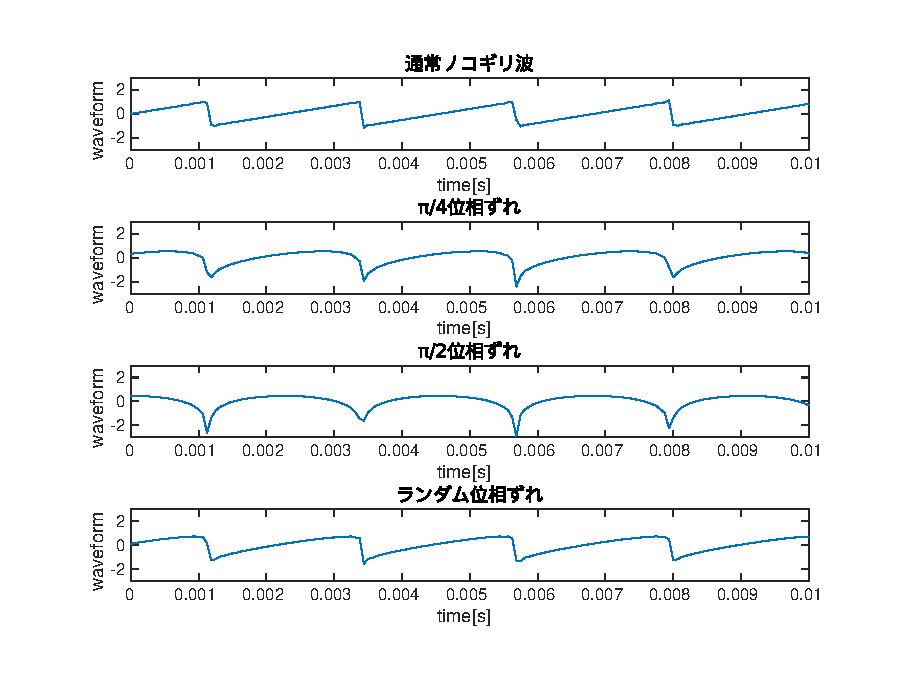
\includegraphics[scale=0.4]{../eps/kadai1_1.eps}
  \end{minipage}
  \begin{minipage}{0.45\linewidth}
    \centering
    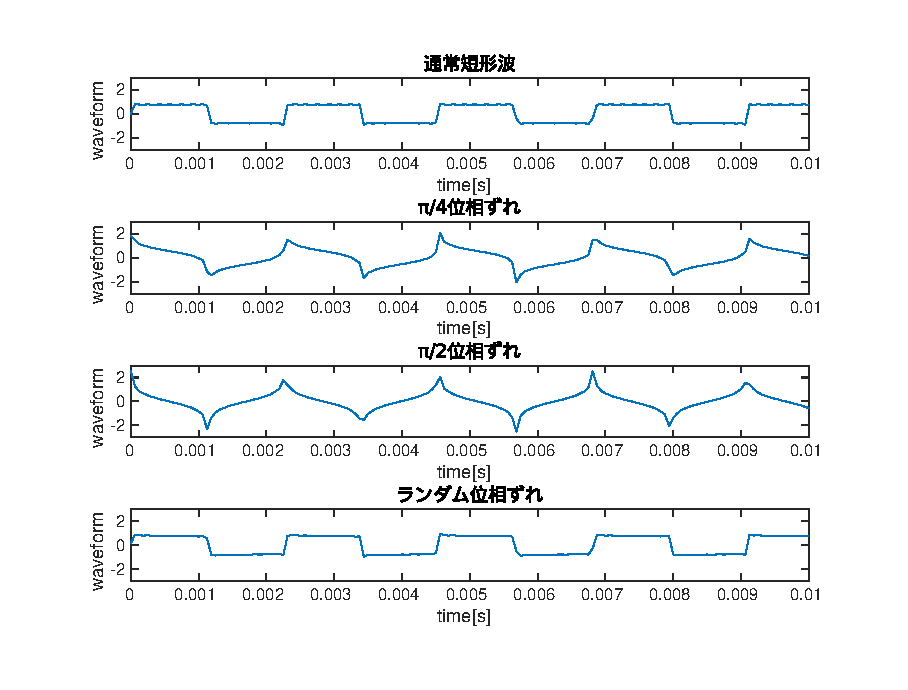
\includegraphics[scale=0.4]{../eps/kadai1_2.eps}
  \end{minipage}
\end{figure}

\clearpage
